\documentclass{beamer}
\usetheme{Copenhagen}
\usepackage{flexiprogram}
\usepackage{wrapfig}
\usepackage[usenames,dvipsnames]{pstricks}
\usepackage{epsfig}
\usepackage{pst-func}
\usepackage{pst-grad} % For gradients
\usepackage{pst-plot} % For axes
\usepackage{pst-node}
\usepackage{url}
\usepackage{ulem}
%\usepackage{enumerate}

% \usepackage[labelfont={bf}]{caption}

\bibliographystyle{plain}

\title{Android Based Greenhouse Monitoring (And Harvesting) Using Accurate And Automated Bot Guidance System}
\author{Devendra Bhave (114050004) \\ \and Mohd Vasimuddin (114050007) \\ \and Meenakshi Verma (123050014) \\ \and Mukund Lahoti (123050018)}
\date{\today}

\setbeamertemplate{footline}[frame number]

\begin{document}

\frame{\titlepage}

\frame{\frametitle{Contents}\tableofcontents} 

\section{Problem Statement}

\frame{\frametitle{Functional Requirements}
Automated Bot Guidance System:
\begin{enumerate}
 \item Maneuver the Bot automatically
 \item Support \alert{\texttt{goto(x, y)}} primitive
 \item {\color{rgb:green,2;black,1} Guarantee accuracy}
\end{enumerate}
}

\frame{\frametitle{Functional Requirements}
Greenhouse Management:
 \only<1> {
\begin{enumerate}
 \item \alert{Semi automatic greenhouse monitoring}
 \item \alert{Semi automatic harvesting}
 \end{enumerate}
 }
 
 \only<2> {
 \begin{enumerate}
 \item \alert{\sout{Semi} automatic greenhouse monitoring}
 \item \alert{Semi automatic harvesting}
 \end{enumerate}
 }
 
 \only<3> {
 \begin{enumerate}
 \item \alert{\sout{Semi}} {\color{rgb:green,2;black,1} automatic greenhouse monitoring}
 \item \alert{Semi automatic harvesting}
 \end{enumerate}
 }
 
 \only<4> {
 \begin{enumerate}
 \item \alert{\sout{Semi}} {\color{rgb:green,2;black,1} automatic greenhouse monitoring}
 \item \alert{\sout{Semi} automatic harvesting}
 \end{enumerate}
 }
 
 \only<5> {
 \begin{enumerate}
 \item \alert{\sout{Semi}} {\color{rgb:green,2;black,1} automatic greenhouse monitoring}
 \item \alert{\sout{Semi}} {\color{rgb:green,2;black,1} automatic harvesting}
 \end{enumerate}
 }
}

\section{System Description}


\frame{\frametitle{Bot Description}
% Generated with LaTeXDraw 2.0.8
% Thu Nov 08 00:11:11 IST 2012
% \usepackage[usenames,dvipsnames]{pstricks}
% \usepackage{epsfig}
% \usepackage{pst-grad} % For gradients
% \usepackage{pst-plot} % For axes
\scalebox{0.7} % Change this value to rescale the drawing.
{
\begin{pspicture}(0,-4.92)(15.8,4.9)
\psframe[linewidth=0.04,dimen=outer](3.6,-0.3)(0.0,-2.5)
\psframe[linewidth=0.04,dimen=outer](5.6,0.7)(2.0,-1.5)
\psarc[linewidth=0.04](3.8,0.7){1.8}{0.0}{180.0}
\psarc[linewidth=0.04](1.8,-0.3){1.8}{0.0}{180.0}
\psline[linewidth=0.04cm](3.6,-2.5)(5.6,-1.5)
\psline[linewidth=0.04cm](3.6,-0.3)(5.6,0.7)
\psline[linewidth=0.04cm](1.0,1.3)(3.0,2.3)
\psline[linewidth=0.04cm](0.0,-2.5)(2.0,-1.5)
\psline[linewidth=0.04cm](0.0,-0.3)(2.0,0.7)
\psline[linewidth=0.04cm](1.8,-1.9)(2.6,-1.9)
\psline[linewidth=0.04cm](1.8,-1.9)(1.8,-2.3)
\psline[linewidth=0.04cm](2.6,-1.9)(2.6,-2.3)
\psline[linewidth=0.04cm](1.8,-2.3)(2.6,-2.3)
\psline[linewidth=0.04cm](1.8,-1.9)(2.2,-1.7)
\psline[linewidth=0.04cm](2.2,-1.7)(3.0,-1.7)
\psline[linewidth=0.04cm](3.0,-1.7)(2.6,-1.9)
\psline[linewidth=0.04cm](3.0,-1.7)(3.0,-2.1)
\psline[linewidth=0.04cm](2.6,-2.3)(3.0,-2.1)
\pscircle[linewidth=0.04,linestyle=dashed,dash=0.16cm 0.16cm,dimen=outer](2.4,-2.1){0.8}
\psline[linewidth=0.04cm](7.0,-0.9)(7.6,-0.3)
\psline[linewidth=0.04cm](11.6,-0.3)(11.0,-0.9)
\psline[linewidth=0.04cm](11.6,-0.3)(11.6,-2.1)
\psline[linewidth=0.04cm](11.6,-2.1)(11.0,-2.7)
\pscircle[linewidth=0.04,dimen=outer](9.1,-2.6){1.1}
\psline[linewidth=0.04cm](10.2,-2.7)(11.0,-2.7)
\psline[linewidth=0.04cm](11.0,-2.7)(11.0,-0.9)
\psline[linewidth=0.04cm](11.0,-0.9)(7.0,-0.9)
\psline[linewidth=0.04cm](7.0,-0.9)(7.0,-2.7)
\psline[linewidth=0.04cm](7.0,-2.7)(8.0,-2.7)
\psarc[linewidth=0.04](9.9,-2.0){1.1}{-80.0}{-40.0}
\psline[linewidth=0.04cm](8.2,2.7)(8.2,0.3)
\psline[linewidth=0.04cm](8.2,2.7)(8.8,3.3)
\psline[linewidth=0.04cm](8.8,3.3)(8.8,0.9)
\psline[linewidth=0.04cm](8.8,0.9)(8.2,0.3)
\psline[linewidth=0.04cm](8.2,2.7)(7.8,2.7)
\psline[linewidth=0.04cm](7.8,2.7)(7.8,0.3)
\psline[linewidth=0.04cm](7.8,2.7)(8.4,3.3)
\psline[linewidth=0.04cm](8.4,3.3)(8.8,3.3)
\psline[linewidth=0.04cm](9.8,0.1)(9.8,-0.7)
\psline[linewidth=0.04cm](10.4,0.1)(10.4,-0.7)
\psline[linewidth=0.04cm](9.8,-0.7)(10.4,-0.7)
\psline[linewidth=0.04cm](10.6,-0.1)(10.6,-0.5)
\psline[linewidth=0.04cm](10.6,-0.5)(10.4,-0.7)
\psline[linewidth=0.04cm](10.6,0.1)(10.6,-0.1)
\psline[linewidth=0.04cm](11.6,-0.3)(10.6,-0.3)
\psline[linewidth=0.04cm](9.8,-0.3)(7.6,-0.3)
\psellipse[linewidth=0.04,dimen=outer](8.5,2.5)(0.1,0.2)
\pscircle[linewidth=0.04,linestyle=dashed,dash=0.16cm 0.16cm,dimen=outer](10.9,0.0){4.9}
\psline[linewidth=0.04cm,linestyle=dashed,dash=0.16cm 0.16cm](2.2,-1.3)(8.2,4.1)
\psline[linewidth=0.04cm,linestyle=dashed,dash=0.16cm 0.16cm](2.2,-2.9)(10.2,-4.9)
\usefont{T1}{ptm}{m}{n}
\rput(9.697344,-1.195){FireBird Bot}
\usefont{T1}{ptm}{m}{n}
\rput(1.6484375,2.405){Greenhouse}
\usefont{T1}{ptm}{m}{n}
\rput(11.926094,4.005){Robotic Arm}
\psline[linewidth=0.04cm,arrowsize=0.05291667cm 2.0,arrowlength=1.4,arrowinset=0.4]{->}(11.8,3.7)(11.8,1.7)
\psline[linewidth=0.04cm](7.6,0.3)(12.0,0.3)
\psline[linewidth=0.04cm](8.8,0.9)(11.4,0.9)
\psline[linewidth=0.04cm](11.8,0.9)(12.4,0.9)
\psline[linewidth=0.04cm](12.4,0.9)(12.0,0.3)
\psline[linewidth=0.04cm](7.6,0.3)(7.8,0.5)
\psline[linewidth=0.04cm](7.6,0.3)(7.6,0.1)
\psline[linewidth=0.04cm](7.6,0.1)(12.0,0.1)
\psline[linewidth=0.04cm](12.0,0.3)(12.0,0.1)
\psline[linewidth=0.04cm](12.4,0.9)(12.4,0.7)
\psline[linewidth=0.04cm](12.4,0.7)(12.0,0.1)
\pspolygon[linewidth=0.04,fillstyle=solid](11.4,0.7)(12.6,2.9)(12.8,2.9)(11.8,0.7)
\pspolygon[linewidth=0.04,fillstyle=solid](11.2,0.5)(12.4,2.7)(12.6,2.7)(11.6,0.5)
\psframe[linewidth=0.04,dimen=outer,fillstyle=solid](13.0,2.9)(12.2,2.7)
\pspolygon[linewidth=0.04](12.6,2.9)(13.6,3.5)(13.0,2.9)
\pspolygon[linewidth=0.04](13.0,2.9)(14.0,3.3)(13.0,2.7)
\usefont{T1}{ptm}{m}{n}
\rput(14.107187,1.405){Cutters}
\usefont{T1}{ptm}{m}{n}
\rput(9.575,4.005){IP Camera}
\psline[linewidth=0.04cm,arrowsize=0.05291667cm 2.0,arrowlength=1.4,arrowinset=0.4]{->}(14.0,1.7)(13.4,2.7)
\psline[linewidth=0.04cm,arrowsize=0.05291667cm 2.0,arrowlength=1.4,arrowinset=0.4]{->}(9.6,3.7)(9.0,3.3)
\psframe[linewidth=0.04,dimen=outer,fillstyle=solid](13.6,-1.3)(11.0,-2.7)
\psline[linewidth=0.04cm](14.2,-0.7)(13.6,-1.3)
\psline[linewidth=0.04cm](14.2,-2.1)(13.6,-2.7)
\psline[linewidth=0.04cm](11.6,-0.7)(14.2,-0.7)
\psline[linewidth=0.04cm](14.2,-0.7)(14.2,-2.1)
\usefont{T1}{ptm}{m}{n}
\rput(14.438125,0.605){Fruit Collector}
\psline[linewidth=0.04cm,arrowsize=0.05291667cm 2.0,arrowlength=1.4,arrowinset=0.4]{->}(14.2,0.3)(13.2,-0.7)
\end{pspicture} 
}

}

\frame{\frametitle{System Architecture}
 % Generated with LaTeXDraw 2.0.8
% Thu Nov 08 00:26:46 IST 2012
% \usepackage[usenames,dvipsnames]{pstricks}
% \usepackage{epsfig}
% \usepackage{pst-grad} % For gradients
% \usepackage{pst-plot} % For axes
\scalebox{0.7} % Change this value to rescale the drawing.
{
\begin{pspicture}(0,-2.5)(15.780625,2.5)
\usefont{T1}{ptm}{m}{n}
\rput(5.1175,-1.935){Firebird}
\usefont{T1}{ptm}{m}{n}
\rput(0.76234376,-0.995){ADC}
\usefont{T1}{ptm}{m}{n}
\rput(2.108125,-0.995){Buzzer}
\usefont{T1}{ptm}{m}{n}
\rput(3.5495312,-0.995){LCD}
\usefont{T1}{ptm}{m}{n}
\rput(4.848125,-0.995){Motor}
\usefont{T1}{ptm}{m}{n}
\rput(6.268125,-0.995){Power}
\usefont{T1}{ptm}{m}{n}
\rput(7.6025,-0.995){Servo}
\usefont{T1}{ptm}{m}{n}
\rput(9.0725,-0.995){Zigbee}
\psframe[linewidth=0.04,dimen=outer](9.8,-0.5)(0.0,-1.5)
\psline[linewidth=0.04cm](8.4,-0.5)(8.4,-1.5)
\psline[linewidth=0.04cm](7.0,-0.5)(7.0,-1.5)
\psline[linewidth=0.04cm](5.6,-0.5)(5.6,-1.5)
\psline[linewidth=0.04cm](4.2,-0.5)(4.2,-1.5)
\psline[linewidth=0.04cm](2.8,-0.5)(2.8,-1.5)
\psline[linewidth=0.04cm](1.4,-0.5)(1.4,-1.5)
\psframe[linewidth=0.04,dimen=outer](9.8,-1.5)(0.0,-2.5)
\psframe[linewidth=0.04,dimen=outer](9.8,0.5)(0.0,-0.5)
\psline[linewidth=0.04cm](5.0,-0.5)(5.0,0.5)
\usefont{T1}{ptm}{m}{n}
\rput(2.5323439,0.005){Assertions}
\usefont{T1}{ptm}{m}{n}
\rput(7.262656,0.005){AVR-libc}
\psframe[linewidth=0.04,dimen=outer](9.8,1.5)(0.0,0.5)
\psline[linewidth=0.04cm](5.0,1.5)(5.0,0.5)
\usefont{T1}{ptm}{m}{n}
\rput(2.4160938,1.005){ROM Filesystem}
\usefont{T1}{ptm}{m}{n}
\rput(7.55875,1.005){Whiteline Follower}
\psframe[linewidth=0.04,dimen=outer](9.8,2.5)(0.0,1.5)
\usefont{T1}{ptm}{m}{n}
\rput(4.96625,2.005){Bot Guidance System}
\usefont{T1}{ptm}{m}{n}
\rput(11.297344,-1.995){Hardware}
\usefont{T1}{ptm}{m}{n}
\rput(13.165,-0.995){Hardware Abstraction Layer (HAL)}
\usefont{T1}{ptm}{m}{n}
\rput(11.891875,0.005){Software Libraries}
\usefont{T1}{ptm}{m}{n}
\rput(11.1328125,1.005){Utilities}
\usefont{T1}{ptm}{m}{n}
\rput(11.406875,2.005){Application}
\end{pspicture} 
}

}

\frame{\frametitle{Hardware Abstraction Layer (HAL)}
 Offers functionality specific interfaces
 
 \vspace{\baselineskip}
 
 Provides \texttt{init}$<$ModuleName$>$\texttt{()} interface for module initialization 
 
}

\frame{\frametitle{HAL -- ADC, Buzzer}
Interfaces:

\begin{itemize}
 \item \texttt{initAdc()}
 \begin{itemize}
  \item Initialize ADC hardware
 \end{itemize}
 \item \texttt{getAdcValue(adc\_channel)}
 \begin{itemize}
  \item Read ADC value for specified channel
 \end{itemize} 
\end{itemize}

\vspace{\baselineskip}
\begin{itemize}
 \item \texttt{initBuzzer()}
 \begin{itemize}
  \item Initialize ADC hardware
 \end{itemize}
 \item \texttt{buzzerOn()}
 \begin{itemize}
  \item Turn on buzzer
 \end{itemize}
 \item \texttt{buzzerOff()}
 \begin{itemize}
  \item Turn off buzzer
 \end{itemize} 
\end{itemize} 
}

\frame{\frametitle{HAL -- LCD}
Interfaces:

\begin{itemize}
 \item \texttt{initLcd()}
 \begin{itemize}
  \item Initialize LCD hardware
 \end{itemize}
 \item \texttt{lcdHome()}
 \begin{itemize}
  \item Place cursor at first column on LCD display
 \end{itemize}
 \item \texttt{lcdClear()}
 \begin{itemize}
  \item Clear LCD screen
 \end{itemize} 
 \item \texttt{lcdCursor(row, column)}
 \begin{itemize}
  \item Place cursor at given row and column on LCD display
 \end{itemize} 
 \item \texttt{lcdString(data)}
 \begin{itemize}
  \item Write data on LCD display
 \end{itemize} 
\end{itemize}
}

\frame{\frametitle{HAL -- Motor}
\begin{itemize}
 \item \texttt{initMotor()}
 \begin{itemize}
  \item Initialize DC motor hardware
 \end{itemize}
 \item \texttt{motorDirectionSet(direction)}
 \begin{itemize}
  \item Controls DC motors for direction
 \end{itemize}
 \item \texttt{motorVelocitySet(left\_vel, right\_vel)}
 \begin{itemize}
  \item Set motor velocity using PWM
 \end{itemize} 
 \item \texttt{motorVelocityGet()}
 \begin{itemize}
  \item Read motor velocity settings
 \end{itemize} 
 \item \texttt{motorLeftPositionEncoderInit(lCallback)}
 \begin{itemize}
  \item Register left positional encoder callback
 \end{itemize} 
 \item \texttt{motorRightPositionEncoderInit(rCallback)}
 \begin{itemize}
  \item Register right positional encoder callback
 \end{itemize}
 \item \texttt{motorLeftPositionEncoderInterruptConfig(state)}
 \begin{itemize}
  \item Enable/disable left positional encoder interrupt
 \end{itemize}
 \item \texttt{motorRightPositionEncoderInterruptConfig(state)}
 \begin{itemize}
  \item Enable/disable right positional encoder interrupt
 \end{itemize}
 \end{itemize}
}

\frame{\frametitle{HAL -- Power}
Sensor groups:
\begin{enumerate}
 \item \texttt{SG\_GROUP1}: Sharp IR range sensors 2,3,4 and white line LEDs
 \item \texttt{SG\_GROUP2}: Sharp IR range sensors 1,5
 \item \texttt{SG\_GROUP3}: IR proximity sensors
\end{enumerate}

\vspace{\baselineskip}
\begin{itemize}
 \item \texttt{initPower()}
 \begin{itemize}
  \item Initialize power management hardware
 \end{itemize}
 \item \texttt{powerOn(sensor\_group)}
 \begin{itemize}
  \item Turns power on for given group of sensors
 \end{itemize}
 \item \texttt{powerOff(sensor\_group)}
 \begin{itemize}
  \item Turns power off for given group of sensors
 \end{itemize} 
\end{itemize} 
 }

 \frame{\frametitle{HAL -- Servo}
\begin{itemize}
 \item \texttt{initServo()}
 \begin{itemize}
  \item Initialize servo motor hardware
 \end{itemize}
 \item \texttt{servoSet(motor, angle)}
 \begin{itemize}
  \item Sets given angle for servo motor
 \end{itemize}
 \item \texttt{servoFree(motor)}
 \begin{itemize}
  \item Unlocks servo motors
 \end{itemize} 
\end{itemize} 
 }

\frame{\frametitle{Assertions}
 Offers facitily on Firebird for assertion based debugging
 
 \vspace{\baselineskip}
 
 Use \texttt{ASSERT(condition)} in the code
 
 \vspace{\baselineskip}
 
 If condition fails
 \begin{itemize}
  \item bot halts and beeps continuously
  \item displays line number, filename and failed condition on LCD screen
 \end{itemize}
 
 \vspace{\baselineskip}
 
 Assertions are replaced by \structure{empty statements} when not debugging.
}

\frame{\frametitle{ROM Filesystem}
 No filesystem support in AVR libc. So, we \alert{wrote our own}.
 
 \vspace{\baselineskip}
 Map file for bot guidance system can be added at compile time.
 
 \vspace{\baselineskip}
 Map file can be accessed using file handle \texttt{MAP\_FILE} for \texttt{fscanf()},
 \texttt{fgets()}, etc.
 
 \vspace{\baselineskip}
 Standard file streams (STDIN, STDOUT) are redirected to Zigbee. \texttt{printf()}, \texttt{scanf()} used anywhere in
 code sends or receives data over Zigbee.
 
 \vspace{\baselineskip}
 \structure{Greenhouse map can be loaded at runtime.}
}

\frame{\frametitle{Whiteline Follower}
Suppoted primitives:

 \vspace{\baselineskip}
\begin{itemize}
 \item \texttt{moveForwardFollwingLineByDistance(distance)}
 \begin{itemize}
  \item Moves along whiteline till specified distance is covered
 \end{itemize} 
 \item \texttt{moveForwardFollwingLineByCheckpoint(exp\_dist)}
 \begin{itemize}
  \item Moves along whiteline until checkpoint is hit
 \end{itemize} 
 \item \texttt{rotateBot(direction, angle)}
 \begin{itemize}
  \item Rotates bot in specified direction by given degrees
 \end{itemize} 
\end{itemize} 

}

\frame{\frametitle{Checkpoint Synchronization Automaton}
% Generated with LaTeXDraw 2.0.8
% Thu Nov 08 01:30:12 IST 2012
% \usepackage[usenames,dvipsnames]{pstricks}
% \usepackage{epsfig}
% \usepackage{pst-grad} % For gradients
% \usepackage{pst-plot} % For axes
\scalebox{0.7} % Change this value to rescale the drawing.
{
\begin{pspicture}(0,-4.408125)(15.7890625,4.408125)
\usefont{T1}{ptm}{m}{n}
\rput(2.501875,1.4146875){\psframebox[linewidth=0.04]{Outside Checkpoint Range}}
\usefont{T1}{ptm}{m}{n}
\rput(10.635938,2.6146874){Within Checkpoint Range}
\usefont{T1}{ptm}{m}{n}
\rput(12.367344,-1.3853126){Checkpoint Missed}
\usefont{T1}{ptm}{m}{n}
\rput(2.7435937,-1.3853126){Unexpected Checkpoint Error}
\usefont{T1}{ptm}{m}{n}
\rput(7.8323436,-1.3853126){At Checkpoint}
\psarc[linewidth=0.04,arrowsize=0.05291667cm 2.0,arrowlength=1.4,arrowinset=0.4]{->}(3.0934374,1.6096874){0.7}{0.0}{180.0}
\psframe[linewidth=0.04,dimen=outer](12.593437,3.1096876)(8.593437,2.3096876)
\rput{-45.0}(0.6624435,8.418655){\psarc[linewidth=0.04,arrowsize=0.05291667cm 2.0,arrowlength=1.4,arrowinset=0.4]{->}(10.493438,3.4096875){0.5}{0.0}{270.0}}
\psframe[linewidth=0.04,dimen=outer](13.993438,-0.8903125)(10.793438,-1.6903125)
\psframe[linewidth=0.04,dimen=outer](8.993438,-0.8903125)(6.5934377,-1.6903125)
\psframe[linewidth=0.04,dimen=outer](4.9934373,-0.8903125)(0.3934375,-1.6903125)
\psline[linewidth=0.04cm,arrowsize=0.05291667cm 2.0,arrowlength=1.4,arrowinset=0.4]{->}(4.5934377,1.5096875)(8.593437,2.7096875)
\psline[linewidth=0.04cm,arrowsize=0.05291667cm 2.0,arrowlength=1.4,arrowinset=0.4]{->}(10.993438,2.3096876)(12.393437,-0.8903125)
\psline[linewidth=0.04cm,arrowsize=0.05291667cm 2.0,arrowlength=1.4,arrowinset=0.4]{->}(10.993438,2.3096876)(7.9934373,-0.8903125)
\psline[linewidth=0.04cm,arrowsize=0.05291667cm 2.0,arrowlength=1.4,arrowinset=0.4]{->}(2.3934374,1.1096874)(1.5934376,-0.8903125)
\usefont{T1}{ptm}{m}{n}
\rput(0.961875,-2.5853126){Legend:}
\usefont{T1}{ptm}{m}{n}
\rput(2.1284375,-2.9853125){D: Distance covered yet}
\usefont{T1}{ptm}{m}{n}
\rput(2.979375,-3.3853126){$R_L$: Checkpoint range lower bound}
\usefont{T1}{ptm}{m}{n}
\rput(3.009375,-3.7853124){$R_H$: Checkpoint range upper bound}
\usefont{T1}{ptm}{m}{n}
\rput(5.1403127,-4.1853123){C: Checkpoint sensing (1 means checkpoint hit, 0 otherwise)}
\usefont{T1}{ptm}{m}{n}
\rput(1.7079687,2.6146874){<$D < R_L$, $C==0$>}
\usefont{T1}{ptm}{m}{n}
\rput(6.2079687,2.8146875){<$D == R_L$, $C==0$>}
\usefont{T1}{ptm}{m}{n}
\rput(10.827969,4.2146873){<$D <= R_H$, $C==0$>}
\usefont{T1}{ptm}{m}{n}
\rput(13.967969,0.8146875){<$D > R_H$, $C==X$>}
\usefont{T1}{ptm}{m}{n}
\rput(1.7079687,0.2146875){\psframebox*[framesep=0, boxsep=false,fillcolor=white] {<$D < R_L$, $C==1$>}}
\usefont{T1}{ptm}{m}{n}
\rput(9.027968,1.0146875){\psframebox*[framesep=0, boxsep=false,fillcolor=white] {<$D <= R_H$, $C==1$>}}
\psline[linewidth=0.04cm,arrowsize=0.05291667cm 2.0,arrowlength=1.4,arrowinset=0.4]{->}(3.5934374,1.1096874)(6.9934373,-0.8903125)
\usefont{T1}{ptm}{m}{n}
\rput(6.007969,-0.1853125){\psframebox*[framesep=0, boxsep=false,fillcolor=white] {<$D == R_L$, $C==1$>}}
\end{pspicture} 
}

}

\frame{\frametitle{Bot Guidance System}
Design summary:
\begin{itemize}
 \item Map of arena is precisely known
 \item Use white line to follow shortest path to destination from current location
 \item Add checkpoints to mitigate location errors
\end{itemize}

\vspace{\baselineskip}
\pause
Suppoted primitives:
\begin{itemize}
 \item \texttt{gotoPosition(x, y)}
 \begin{itemize}
  \item x and y are destination co-ordinates in millimeters
 \end{itemize} 
 \item \texttt{setBotOrientation(orientation)}
 \begin{itemize}
  \item Changes bot orientation
 \end{itemize} 
\end{itemize}
 
}

\frame{\frametitle{Bot Guidance System}
Features:

\begin{itemize}
 \item Precomputes all node shortest paths using Floyd-Warshall algorithm
 \item Uses integer only computations for speed
 \item Uses fast integer square roots
 \item Assertion based validation
 \item \alert{Loop invariants analysis and testing using assertions} -- first step towards \structure{formal verification}
 \item Exhaustive test procedures
\end{itemize}
}

\frame{\frametitle{Linux Applications}
Harvesting and monitoring tasks are simple Linux applications.

\vspace{\baselineskip}
\structure{Harvesting}:
\begin{itemize}
 \item Use \texttt{gotoPosition()} primitive to move to desired trough
 \item Use CURL to fetch image from IP camera
 \item Use OpenCV to process image and detect cuttera and fruits
 \item Control Bot over Zigbee to adjust cutter and cut fruits
\end{itemize}

\structure{Monitoring}:
\begin{itemize}
 \item Use \texttt{gotoPosition()} primitive to move to desired trough
 \item Use CURL to fetch images from IP camera
 \item Save images for user to view
\end{itemize}

}

\section{Energy Analysis}
\frame{\frametitle{Battery Levels}
With repeated experiments, we have defined following battery levels.

\vspace{\baselineskip}
\begin{tabular}{|c|c|l|}
 \hline
 Battery Voltage & Battery API value & Meaning\\
 \hline
 \hline
 9.0 V & $> 900$ & Battery is sufficiently charged.\\
 \hline
 8.0 V & $< 800$ & Battery is low\\
 & & Do not start new task.\\
 & & Finish current task.\\
 \hline
 7.5 V & $< 750$ &  Battery is critically low.\\
 & & Abandon current task.\\
 & & Turn off all servo motors\\
 & & Run towards recharge station.\\
 \hline
\end{tabular}

}

\frame{\frametitle{Energy Statistics}
\begin{tabular}{|l|l|l|}
 \hline
 Action & Energy (Watt-Sec) & Energy (Watt-Hr)\\
 \hline
 \hline
 Move Bot along whiteline & 358 per meter & 0.01 per meter\\
 \hline
 Cutter and arm movement & &\\
 + move forward by 10cm & 340 & 0.094\\
 \hline
 Scan sideways for fruits & 1326 & 0.368\\
 \hline
 Cutting fruit & 1029 per fruit & 0.286 per fruit\\
 \hline
 One trajectory & 2875 & 0.799\\
 \hline
 One trough & &  \\
 (= 5 trajectories)& 14375 & 3.99\\
 \hline
 \end{tabular}
 
}






















\frame{\frametitle{Source of Error in Detecting Checkpoint}
Checkpoint sensing is not perfect. It introduces small amount of location error $\epsilon$.

\vspace{\baselineskip}
This error is due to delay between instant when the Bot passes over checkpoint and the instant when
guidance system updates Bot location.

\vspace{\baselineskip}
If Bot is moving with speed 10 cm/sec and delay in updating its location is 20 msec, error $\epsilon$ is 2 mm.
}

\frame{\frametitle{Error Characteristics Of Bot Guidance System}
% Generated with LaTeXDraw 2.0.8
% Thu Sep 27 23:22:19 IST 2012
% \usepackage[usenames,dvipsnames]{pstricks}
% \usepackage{epsfig}
% \usepackage{pst-grad} % For gradients
% \usepackage{pst-plot} % For axes
\scalebox{1} % Change this value to rescale the drawing.
{
\begin{pspicture}(0,-1.3417188)(6.6140623,1.3217187)
\definecolor{color373}{rgb}{0.9411764705882353,0.0,0.0}
\psline[linewidth=0.04cm,arrowsize=0.05291667cm 2.0,arrowlength=1.4,arrowinset=0.4]{<-}(0.6628125,1.3017187)(0.6628125,-0.6982812)
\psline[linewidth=0.04cm,arrowsize=0.05291667cm 2.0,arrowlength=1.4,arrowinset=0.4]{->}(0.6628125,-0.6982812)(5.2628126,-0.6982812)
\psline[linewidth=0.04cm](0.6628125,-0.29828125)(2.4628124,1.1017188)
\psline[linewidth=0.04cm](2.4628124,1.1017188)(2.4628124,-0.29828125)
\psline[linewidth=0.04cm](2.4628124,-0.29828125)(3.4628124,0.50171876)
\psline[linewidth=0.04cm](3.4628124,0.50171876)(3.4628124,-0.29828125)
\psline[linewidth=0.04cm](3.4628124,-0.29828125)(4.8628125,0.90171874)
\psline[linewidth=0.04cm](4.8628125,0.90171874)(4.8628125,-0.29828125)
\psdots[dotsize=0.2,linecolor=color373](2.4628124,-0.6982812)
\psdots[dotsize=0.2,linecolor=color373](3.4628124,-0.6982812)
\psdots[dotsize=0.2,linecolor=color373](4.8628125,-0.6982812)
\psdots[dotsize=0.2,linecolor=color373](0.6628125,-0.6982812)
\psline[linewidth=0.04cm,linestyle=dotted,dotsep=0.16cm](0.6628125,-0.29828125)(5.2628126,-0.29828125)
\psline[linewidth=0.04cm,linestyle=dotted,dotsep=0.16cm](0.6628125,1.1017188)(5.2628126,1.1017188)
\usefont{T1}{ptm}{m}{n}
\rput{-270.0}(0.35171875,0.09671876){\rput(0.1203125,0.20671874){Location Error}}
\usefont{T1}{ptm}{m}{n}
\rput(2.78875,-1.1932813){Path}
\psline[linewidth=0.04cm](5.4628124,-0.29828125)(5.8628125,-0.29828125)
\psline[linewidth=0.04cm](5.4628124,-0.6982812)(5.8628125,-0.6982812)
\psline[linewidth=0.04cm,arrowsize=0.05291667cm 2.0,arrowlength=1.4,arrowinset=0.4]{<-}(5.6628127,-0.6982812)(5.6628127,-1.0982813)
\psline[linewidth=0.04cm,arrowsize=0.05291667cm 2.0,arrowlength=1.4,arrowinset=0.4]{->}(5.6628127,0.10171875)(5.6628127,-0.29828125)
\usefont{T1}{ptm}{m}{n}
\rput(5.6628127,-0.49328125){$\epsilon$}
\psline[linewidth=0.04cm,arrowsize=0.05291667cm 2.0,arrowlength=1.4,arrowinset=0.4]{<-}(6.4628124,1.1017188)(6.4628124,0.50171876)
\psline[linewidth=0.04cm,arrowsize=0.05291667cm 2.0,arrowlength=1.4,arrowinset=0.4]{->}(6.4628124,0.10171875)(6.4628124,-0.6982812)
\usefont{T1}{ptm}{m}{n}
\rput(6.5139065,0.30671874){$\delta_{max}$}
\end{pspicture} 
}

\vspace{\baselineskip}
\begin{itemize}
 \item Minimum location error present at any time is constant $\epsilon$
 \item Maximum location error that may occur is constant $\delta_{max}$
 \item $\epsilon \ll \delta_{max}$
\end{itemize}
}

\frame{\frametitle{Precision Of Bot Guidance System}

\vspace{\baselineskip}
Let, $D_{max}$ be maximum distance between two consecutive checkpoints along any path

\vspace{\baselineskip}
$\therefore \delta_{max} = \kappa \cdot D_{max}$

\vspace{\baselineskip}
Note that $\delta_{max}$ is constant for given placement of checkpoints. Thus, upper bound on error is \alert{constant}.
}

\frame{\frametitle{Error Tolerance Of Bot Guidance System}
Let, $D_{min}$ be minimum distance between two consecutive checkpoints along any path

\vspace{\baselineskip}

% Generated with LaTeXDraw 2.0.8
% Fri Sep 28 00:02:34 IST 2012
% \usepackage[usenames,dvipsnames]{pstricks}
% \usepackage{epsfig}
% \usepackage{pst-grad} % For gradients
% \usepackage{pst-plot} % For axes
\scalebox{1} % Change this value to rescale the drawing.
{
\begin{pspicture}(0,-1.2789062)(5.7,1.2589062)
\definecolor{color373}{rgb}{0.9411764705882353,0.0,0.0}
\psline[linewidth=0.04cm](0.1,-0.26109374)(4.7,-0.26109374)
\psdots[dotsize=0.2,linecolor=color373](0.1,-0.26109374)
\psframe[linewidth=0.04,dimen=outer](3.1,0.5389063)(2.7,-0.06109375)
\psframe[linewidth=0.04,dimen=outer](5.7,1.2389063)(2.9,0.63890624)
\psline[linewidth=0.04cm](2.9,0.5389063)(2.9,-0.26109374)
\psline[linewidth=0.04cm](4.3,-0.26109374)(4.3,1.2389063)
\psdots[dotsize=0.2,linecolor=color373](2.9,-0.26109374)
\psdots[dotsize=0.2,linecolor=color373](4.3,-0.26109374)
\usefont{T1}{ptm}{m}{n}
\rput(3.5560937,-1.0560937){$D_{min}$}
\psline[linewidth=0.04cm,tbarsize=0.07055555cm 5.0]{|-|}(2.9,-0.6610938)(4.3,-0.6610938)
\end{pspicture} 
}

\vspace{\baselineskip}
Error tolerance is upto $D_{min}$.

\vspace{\baselineskip}
Maximize $D_{min}$ to increase error tolerance, but minimize $D_{max}$ to improve accuracy.

$D_{max} = D_{min}$ is optimal design choice.
}

\frame{\frametitle{Correctness Parameters of Bot Guidance System}
\begin{itemize}
 \item \structure{Accuracy}: $\epsilon$
 \item \structure{Precision}: $\delta_{max}$ 
 \item \structure{Error Tolerance}: $< D_{min}$ 
\end{itemize}

}

\frame{\frametitle{Implementation of Checkpoints}
Desired properties of checkpoint:
\begin{itemize}
 \item Should be immovable
 \item Should be inexpensive
 \item Should need minimum additional hardware for detection
 \item Should consume as low power as possible
  \item Bot must detect it reliably
\end{itemize}

\vspace{\baselineskip}
\pause

Recall that for white line follower, left sensor = White, middle sensor = Black, right sensor = White is \alert{impossible}
entry.

\vspace{\baselineskip}
\pause
That's our checkpoint!
}

\frame{\frametitle{Implementation of Checkpoints}
% Generated with LaTeXDraw 2.0.8
% Fri Sep 28 00:24:03 IST 2012
% \usepackage[usenames,dvipsnames]{pstricks}
% \usepackage{epsfig}
% \usepackage{pst-grad} % For gradients
% \usepackage{pst-plot} % For axes
\scalebox{1} % Change this value to rescale the drawing.
{
\begin{pspicture}(0,-3.2)(10.0,3.2)
\definecolor{color373}{rgb}{0.9411764705882353,0.0,0.0}
\definecolor{color5b}{rgb}{0.0,0.9215686274509803,0.0}
\psframe[linewidth=0.04,dimen=outer,fillstyle=solid,fillcolor=darkgray](10.0,3.2)(0.0,-3.2)
\psframe[linewidth=0.04,dimen=outer,fillstyle=solid,fillcolor=color5b](3.0,2.2)(1.0,1.4)
\psframe[linewidth=0.04,linecolor=white,dimen=outer,fillstyle=solid](9.6,2.8)(0.4,2.6)
\psframe[linewidth=0.04,linecolor=white,dimen=outer,fillstyle=solid](0.6,2.8)(0.4,-2.8)
\psframe[linewidth=0.04,linecolor=white,dimen=outer,fillstyle=solid](3.6,2.8)(3.4,-2.8)
\psframe[linewidth=0.04,linecolor=white,dimen=outer,fillstyle=solid](6.6,2.8)(6.4,-2.8)
\psframe[linewidth=0.04,linecolor=white,dimen=outer,fillstyle=solid](9.6,2.8)(9.4,-2.8)
\psframe[linewidth=0.04,linecolor=white,dimen=outer,fillstyle=solid](9.6,1.0)(0.4,0.8)
\psframe[linewidth=0.04,linecolor=white,dimen=outer,fillstyle=solid](9.6,-0.8)(0.4,-1.0)
\psframe[linewidth=0.04,linecolor=white,dimen=outer,fillstyle=solid](9.6,-2.6)(0.4,-2.8)
\psframe[linewidth=0.04,dimen=outer,fillstyle=solid,fillcolor=color5b](6.0,2.2)(4.0,1.4)
\psframe[linewidth=0.04,dimen=outer,fillstyle=solid,fillcolor=color5b](9.0,2.2)(7.0,1.4)
\psframe[linewidth=0.04,dimen=outer,fillstyle=solid,fillcolor=color5b](3.0,0.4)(1.0,-0.4)
\psframe[linewidth=0.04,dimen=outer,fillstyle=solid,fillcolor=color5b](6.0,0.4)(4.0,-0.4)
\psframe[linewidth=0.04,dimen=outer,fillstyle=solid,fillcolor=color5b](9.0,0.4)(7.0,-0.4)
\psframe[linewidth=0.04,dimen=outer,fillstyle=solid,fillcolor=color5b](3.0,-1.4)(1.0,-2.2)
\psframe[linewidth=0.04,dimen=outer,fillstyle=solid,fillcolor=color5b](6.0,-1.4)(4.0,-2.2)
\psframe[linewidth=0.04,dimen=outer,fillstyle=solid,fillcolor=color5b](9.0,-1.4)(7.0,-2.2)
\psframe[linewidth=0.04,linecolor=color373,dimen=outer,fillstyle=solid,fillcolor=color373](0.6,1.6)(0.4,1.4)
\psframe[linewidth=0.04,linecolor=color373,dimen=outer,fillstyle=solid,fillcolor=color373](3.0,2.8)(2.8,2.6)
\psframe[linewidth=0.04,linecolor=color373,dimen=outer,fillstyle=solid,fillcolor=color373](6.6,2.0)(6.4,1.8)
\psframe[linewidth=0.04,linecolor=color373,dimen=outer,fillstyle=solid,fillcolor=color373](4.2,1.0)(4.0,0.8)
\psframe[linewidth=0.04,linecolor=color373,dimen=outer,fillstyle=solid,fillcolor=color373](0.6,-1.4)(0.4,-1.6)
\psframe[linewidth=0.04,linecolor=color373,dimen=outer,fillstyle=solid,fillcolor=color373](3.6,-2.2)(3.4,-2.4)
\psframe[linewidth=0.04,linecolor=color373,dimen=outer,fillstyle=solid,fillcolor=color373](8.8,2.8)(8.6,2.6)
\psframe[linewidth=0.04,linecolor=color373,dimen=outer,fillstyle=solid,fillcolor=color373](7.2,-0.8)(7.0,-1.0)
\psframe[linewidth=0.04,linecolor=color373,dimen=outer,fillstyle=solid,fillcolor=color373](9.6,0.4)(9.4,0.2)
\psframe[linewidth=0.04,linecolor=color373,dimen=outer,fillstyle=solid,fillcolor=color373](7.4,-2.6)(7.2,-2.8)
\end{pspicture} 
}
}

\frame{\frametitle{Implementation of Checkpoints}
% Generated with LaTeXDraw 2.0.8
% Fri Sep 28 00:24:37 IST 2012
% \usepackage[usenames,dvipsnames]{pstricks}
% \usepackage{epsfig}
% \usepackage{pst-grad} % For gradients
% \usepackage{pst-plot} % For axes
\scalebox{1} % Change this value to rescale the drawing.
{
\begin{pspicture}(0,-3.2)(10.0,3.2)
\definecolor{color5b}{rgb}{0.0,0.9215686274509803,0.0}
\psframe[linewidth=0.04,dimen=outer,fillstyle=solid,fillcolor=darkgray](10.0,3.2)(0.0,-3.2)
\psframe[linewidth=0.04,dimen=outer,fillstyle=solid,fillcolor=color5b](3.0,2.2)(1.0,1.4)
\psframe[linewidth=0.04,linecolor=white,dimen=outer,fillstyle=solid](9.6,2.8)(0.4,2.6)
\psframe[linewidth=0.04,linecolor=white,dimen=outer,fillstyle=solid](0.6,2.8)(0.4,-2.8)
\psframe[linewidth=0.04,linecolor=white,dimen=outer,fillstyle=solid](3.6,2.8)(3.4,-2.8)
\psframe[linewidth=0.04,linecolor=white,dimen=outer,fillstyle=solid](6.6,2.8)(6.4,-2.8)
\psframe[linewidth=0.04,linecolor=white,dimen=outer,fillstyle=solid](9.6,2.8)(9.4,-2.8)
\psframe[linewidth=0.04,linecolor=white,dimen=outer,fillstyle=solid](9.6,1.0)(0.4,0.8)
\psframe[linewidth=0.04,linecolor=white,dimen=outer,fillstyle=solid](9.6,-0.8)(0.4,-1.0)
\psframe[linewidth=0.04,linecolor=white,dimen=outer,fillstyle=solid](9.6,-2.6)(0.4,-2.8)
\psframe[linewidth=0.04,dimen=outer,fillstyle=solid,fillcolor=color5b](6.0,2.2)(4.0,1.4)
\psframe[linewidth=0.04,dimen=outer,fillstyle=solid,fillcolor=color5b](9.0,2.2)(7.0,1.4)
\psframe[linewidth=0.04,dimen=outer,fillstyle=solid,fillcolor=color5b](3.0,0.4)(1.0,-0.4)
\psframe[linewidth=0.04,dimen=outer,fillstyle=solid,fillcolor=color5b](6.0,0.4)(4.0,-0.4)
\psframe[linewidth=0.04,dimen=outer,fillstyle=solid,fillcolor=color5b](9.0,0.4)(7.0,-0.4)
\psframe[linewidth=0.04,dimen=outer,fillstyle=solid,fillcolor=color5b](3.0,-1.4)(1.0,-2.2)
\psframe[linewidth=0.04,dimen=outer,fillstyle=solid,fillcolor=color5b](6.0,-1.4)(4.0,-2.2)
\psframe[linewidth=0.04,dimen=outer,fillstyle=solid,fillcolor=color5b](9.0,-1.4)(7.0,-2.2)
\psframe[linewidth=0.04,linecolor=darkgray,dimen=outer,fillstyle=solid,fillcolor=darkgray](3.0,2.8)(2.8,2.6)
\psframe[linewidth=0.04,linecolor=white,dimen=outer,fillstyle=solid](2.96,3.0)(2.8,2.84)
\psframe[linewidth=0.04,linecolor=white,dimen=outer,fillstyle=solid](2.96,2.6)(2.8,2.44)
\psframe[linewidth=0.04,linecolor=darkgray,dimen=outer,fillstyle=solid,fillcolor=darkgray](8.8,2.8)(8.6,2.6)
\psframe[linewidth=0.04,linecolor=darkgray,dimen=outer,fillstyle=solid,fillcolor=darkgray](6.6,2.0)(6.4,1.8)
\psframe[linewidth=0.04,linecolor=darkgray,dimen=outer,fillstyle=solid,fillcolor=darkgray](0.6,1.6)(0.4,1.4)
\psframe[linewidth=0.04,linecolor=darkgray,dimen=outer,fillstyle=solid,fillcolor=darkgray](4.2,1.0)(4.0,0.8)
\psframe[linewidth=0.04,linecolor=darkgray,dimen=outer,fillstyle=solid,fillcolor=darkgray](9.6,0.4)(9.4,0.2)
\psframe[linewidth=0.04,linecolor=darkgray,dimen=outer,fillstyle=solid,fillcolor=darkgray](7.2,-0.8)(7.0,-1.0)
\psframe[linewidth=0.04,linecolor=darkgray,dimen=outer,fillstyle=solid,fillcolor=darkgray](7.4,-2.6)(7.2,-2.8)
\psframe[linewidth=0.04,linecolor=darkgray,dimen=outer,fillstyle=solid,fillcolor=darkgray](3.6,-2.2)(3.4,-2.4)
\psframe[linewidth=0.04,linecolor=darkgray,dimen=outer,fillstyle=solid,fillcolor=darkgray](0.6,-1.4)(0.4,-1.6)
\psframe[linewidth=0.04,linecolor=white,dimen=outer,fillstyle=solid](0.76,1.6)(0.6,1.44)
\psframe[linewidth=0.04,linecolor=white,dimen=outer,fillstyle=solid](0.36,1.6)(0.2,1.44)
\psframe[linewidth=0.04,linecolor=white,dimen=outer,fillstyle=solid](4.16,1.2)(4.0,1.04)
\psframe[linewidth=0.04,linecolor=white,dimen=outer,fillstyle=solid](4.16,0.8)(4.0,0.64)
\psframe[linewidth=0.04,linecolor=white,dimen=outer,fillstyle=solid](6.36,2.0)(6.2,1.84)
\psframe[linewidth=0.04,linecolor=white,dimen=outer,fillstyle=solid](6.76,2.0)(6.6,1.84)
\psframe[linewidth=0.04,linecolor=white,dimen=outer,fillstyle=solid](8.76,3.0)(8.6,2.84)
\psframe[linewidth=0.04,linecolor=white,dimen=outer,fillstyle=solid](8.76,2.6)(8.6,2.44)
\psframe[linewidth=0.04,linecolor=white,dimen=outer,fillstyle=solid](7.16,-0.6)(7.0,-0.76)
\psframe[linewidth=0.04,linecolor=white,dimen=outer,fillstyle=solid](7.16,-1.0)(7.0,-1.16)
\psframe[linewidth=0.04,linecolor=white,dimen=outer,fillstyle=solid](9.36,0.4)(9.2,0.24)
\psframe[linewidth=0.04,linecolor=white,dimen=outer,fillstyle=solid](9.76,0.4)(9.6,0.24)
\psframe[linewidth=0.04,linecolor=white,dimen=outer,fillstyle=solid](0.36,-1.4)(0.2,-1.56)
\psframe[linewidth=0.04,linecolor=white,dimen=outer,fillstyle=solid](0.76,-1.4)(0.6,-1.56)
\psframe[linewidth=0.04,linecolor=white,dimen=outer,fillstyle=solid](3.36,-2.2)(3.2,-2.36)
\psframe[linewidth=0.04,linecolor=white,dimen=outer,fillstyle=solid](3.76,-2.2)(3.6,-2.36)
\psframe[linewidth=0.04,linecolor=white,dimen=outer,fillstyle=solid](7.36,-2.4)(7.2,-2.56)
\psframe[linewidth=0.04,linecolor=white,dimen=outer,fillstyle=solid](7.36,-2.8)(7.2,-2.96)
\end{pspicture} 
}
}

\frame{\frametitle{Implementation of Checkpoints}
Desired properties of checkpoint:
\begin{itemize}
  \item {\color{rgb:green,2;black,1}Should be immovable}
 \item {\color{rgb:green,2;black,1}Should be inexpensive}
 \item {\color{rgb:green,2;black,1}Should need minimum additional hardware for detection}
 \item {\color{rgb:green,2;black,1}Should consume as low power as possible}
  \item {\color{orange}Bot must detect it reliably}
\end{itemize}

\vspace{\baselineskip}
%\pause

Recall that for white line follower, left sensor = White, middle sensor = Black, right sensor = White is \alert{impossible}
entry.

\vspace{\baselineskip}
%\pause
That's our checkpoint!
}

\frame{\frametitle{Implementation of Bot Guidance System}
Bot Guidance System has
\begin{itemize}
 \item the map
 \item precise current location of the Bot
 \item initial orientation of the Bot - E, W, N, S
\end{itemize}

We build \alert{automated} Bot guidance system based on graph algorithms to move the Bot to any desired location
along the \emph{white line}.

\vspace{\baselineskip}
It is possible to implement service primitive \alert{\texttt{goto(x, y)}}.
}

\frame{\frametitle{Implementation of Recharge Station}
% Generated with LaTeXDraw 2.0.8
% Fri Sep 28 01:47:12 IST 2012
% \usepackage[usenames,dvipsnames]{pstricks}
% \usepackage{epsfig}
% \usepackage{pst-grad} % For gradients
% \usepackage{pst-plot} % For axes
\scalebox{1} % Change this value to rescale the drawing.
{
\begin{pspicture}(0,-3.1426563)(8.62,3.1226563)
\psline[linewidth=0.04cm](0.0,1.9026562)(1.8,2.7026563)
\psline[linewidth=0.04cm](0.0,1.9026562)(2.6,2.5026562)
\psline[linewidth=0.04cm](1.8,2.7026563)(3.8,3.1026564)
\psline[linewidth=0.04cm](2.6,2.5026562)(3.8,3.1026564)
\psline[linewidth=0.04cm](2.6,2.5026562)(2.6,2.1026564)
\psline[linewidth=0.04cm](3.8,3.1026564)(3.8,2.7026563)
\psline[linewidth=0.04cm](2.6,2.1026564)(3.8,2.7026563)
\psline[linewidth=0.04cm](0.4,1.5026562)(2.6,2.1026564)
\psline[linewidth=0.04cm](0.0,1.9026562)(0.0,-1.8973438)
\psline[linewidth=0.04cm](0.4,1.5026562)(0.4,-1.8973438)
\psline[linewidth=0.04cm](2.0,-1.0973438)(2.0,1.9026562)
\psline[linewidth=0.04cm](0.0,-1.8973438)(0.4,-1.8973438)
\psline[linewidth=0.04cm](0.4,-1.8973438)(2.0,-1.0973438)
\psline[linewidth=0.04cm](3.6,0.70265627)(4.8,1.1026562)
\psline[linewidth=0.04cm](6.6,0.70265627)(7.8,1.1026562)
\psline[linewidth=0.04cm](7.8,1.1026562)(7.8,-0.89734375)
\psline[linewidth=0.04cm](7.8,-0.89734375)(6.6,-1.2973437)
\pscircle[linewidth=0.04,dimen=outer](5.2,-1.0973438){0.8}
\psarc[linewidth=0.04](6.4,-0.89734375){0.6}{220.0}{330.0}
\psline[linewidth=0.04cm](3.6,0.70265627)(6.6,0.70265627)
\psline[linewidth=0.04cm](6.6,0.70265627)(6.6,-1.2973437)
\psline[linewidth=0.04cm](6.6,-1.2973437)(6.0,-1.2973437)
\psline[linewidth=0.04cm](3.6,0.70265627)(3.6,-1.2973437)
\psline[linewidth=0.04cm](3.6,-1.2973437)(4.4,-1.2973437)
\psline[linewidth=0.04cm](4.8,0.90265626)(4.8,2.1026564)
\psline[linewidth=0.04cm](5.0,2.1026564)(5.0,0.90265626)
\psline[linewidth=0.04cm](4.8,0.90265626)(5.0,0.90265626)
\psellipse[linewidth=0.04,dimen=outer](4.9,2.2026563)(0.3,0.1)
\psellipse[linewidth=0.04,dimen=outer](3.2,-0.39734375)(0.2,0.3)
\psline[linewidth=0.04cm](3.4,-0.29734376)(3.6,-0.29734376)
\psline[linewidth=0.04cm](3.6,-0.49734375)(3.4,-0.49734375)
\psline[linewidth=0.04cm](7.8,1.1026562)(5.0,1.1026562)
\psline[linewidth=0.04cm](0.4,-1.8973438)(7.6,-1.8973438)
\psline[linewidth=0.04cm](2.0,-1.0973438)(3.6,-1.0973438)
\psline[linewidth=0.04cm](7.2,-1.0973438)(8.6,-1.0973438)
\psline[linewidth=0.04,fillstyle=crosshatch*,hatchwidth=0.04,hatchangle=60.0](0.6,-1.0973438)(1.8,-0.49734375)(1.8,0.90265626)(0.6,0.30265626)(0.6,-1.0973438)
\psline[linewidth=0.04cm,arrowsize=0.05291667cm 2.0,arrowlength=1.4,arrowinset=0.4]{<-}(5.2,2.1026564)(6.6,2.1026564)
\usefont{T1}{ptm}{m}{n}
\rput(7.166094,2.0076563){Horn}
\usefont{T1}{ptm}{m}{n}
\rput(3.2807813,1.5876563){Tail}
\psline[linewidth=0.04,fillstyle=vlines*,hatchwidth=0.04,hatchangle=0.0](0.64,1.5426563)(0.64,1.8426563)(2.44,2.3226562)(2.46,2.0826561)(0.66,1.6026562)
\psline[linewidth=0.04cm](2.4,2.1026564)(2.0,-2.6973438)
\psline[linewidth=0.04cm](1.2,-0.29734376)(2.0,-2.6973438)
\usefont{T1}{ptm}{m}{n}
\rput(1.9707812,-2.9923437){Metallic Wool Contact Pads}
\psline[linewidth=0.04cm,arrowsize=0.05291667cm 2.0,arrowlength=1.4,arrowinset=0.4]{<-}(3.2,-0.09734375)(3.2,1.3026563)
\end{pspicture} 
}
}

\frame{\frametitle{Bot Operation Modes}
Bot operates in one of the three operation modes:
\begin{enumerate}
 \item \alert{Automatic} - Automatic Bot guidance system controls the Bot
 \item \alert{Manual} - User controls the Bot remotely (Project exists on e-yantra)\cite{eyantra}
 \item \alert{Transition} - Intermediate mode when switching from manual to automatic
\end{enumerate}

Bot status known to automatic guidance system:
\begin{enumerate}
 \item \alert{Automatic} - guidance system knows location and orientation of the Bot
 \item \alert{Manual} - neither location nor orientation of Bot is known to guidance system
 \item \alert{Transition} - guidance system takes user's help to learn current Bot location and orientation
\end{enumerate}

}

\frame{\frametitle{FSM for Bot Operation Modes}
% Generated with LaTeXDraw 2.0.8
% Fri Sep 28 02:06:38 IST 2012
% \usepackage[usenames,dvipsnames]{pstricks}
% \usepackage{epsfig}
% \usepackage{pst-grad} % For gradients
% \usepackage{pst-plot} % For axes
\scalebox{1} % Change this value to rescale the drawing.
{
\begin{pspicture}(0,-1.6784375)(8.070937,1.6384375)
\usefont{T1}{ptm}{m}{n}
\rput(3.7251563,1.1434375){Automatic}
\usefont{T1}{ptm}{m}{n}
\rput(5.91625,-0.8565625){Transition}
\usefont{T1}{ptm}{m}{n}
\rput(1.7357812,-0.8565625){Manual}
\psellipse[linewidth=0.04,dimen=outer](3.6925,1.1384375)(0.9,0.5)
\psellipse[linewidth=0.04,dimen=outer](5.8925,-0.8615625)(0.9,0.7)
\psellipse[linewidth=0.04,dimen=outer](1.7925,-0.8615625)(1.0,0.5)
\psline[linewidth=0.04cm,arrowsize=0.1cm 4.0,arrowlength=3.0,arrowinset=0.4]{->}(3.5925,0.6384375)(1.9925,-0.3615625)
\psline[linewidth=0.04cm,arrowsize=0.1cm 4.0,arrowlength=3.0,arrowinset=0.4]{->}(2.7925,-0.9615625)(4.9925,-0.9615625)
\psline[linewidth=0.04cm,arrowsize=0.1cm 4.0,arrowlength=3.0,arrowinset=0.4]{->}(5.7925,-0.1615625)(3.9925,0.6384375)
\usefont{T1}{ptm}{m}{n}
\rput(1.4890625,0.5434375){Error or user request}
\usefont{T1}{ptm}{m}{n}
\rput(3.701875,-1.4565625){User request}
\usefont{T1}{ptm}{m}{n}
\rput(6.505156,0.5434375){Checkpoint detection}
\end{pspicture} 
}

\vspace{\baselineskip}
\pause
In transition mode, user manually maneuvers the Bot to nearest checkpoint. User tells Bot guidance system which
checkpoint it should expect next. As the Bot passes over the checkpoint, guidance system knows current location 
and orientation and takes the control of the Bot to itself, switching to automatic mode.
}

\section{Functional Requirements}



\section{Risk Analysis}

\frame{\frametitle{Risk Mitigation}
\structure{Risk \#1} Error in checkpoint detection
\begin{itemize}
 \item Automated guidance system knows location of next checkpoint in the path (Say $D$ units away)
 \item Location error is bounded by constant $\delta_{max}$
 \item Next checkpoint must be detected within the range $[D-\delta_{max}, D+\delta_{max}]$
 \item $\textrm{No checkpoint detected till distance} > (D+\delta_{max}) \Rightarrow$ \alert{Missed checkpoint}
 \item $\textrm{checkpoint detected distance} < (D-\delta_{max}) \Rightarrow$ \alert{False checkpoint detection}
\end{itemize}
}

\frame{\frametitle{Risk Mitigation}
 \structure{Risk \#2} Error in white line following
 Certain cases in while following white line are errors. (e.g. all sensors detect black)

\vspace{\baselineskip}
For \structure{Risk \#1} and \structure{Risk \#2}, switch the Bot in manual mode and alert user remotely.
}

\frame{\frametitle{Risk Mitigation}
 \structure{Risk \#3} Battery is low
 
 Go to recharge station and wait there till battery is completely charged.
 \vspace{\baselineskip}
 \pause

  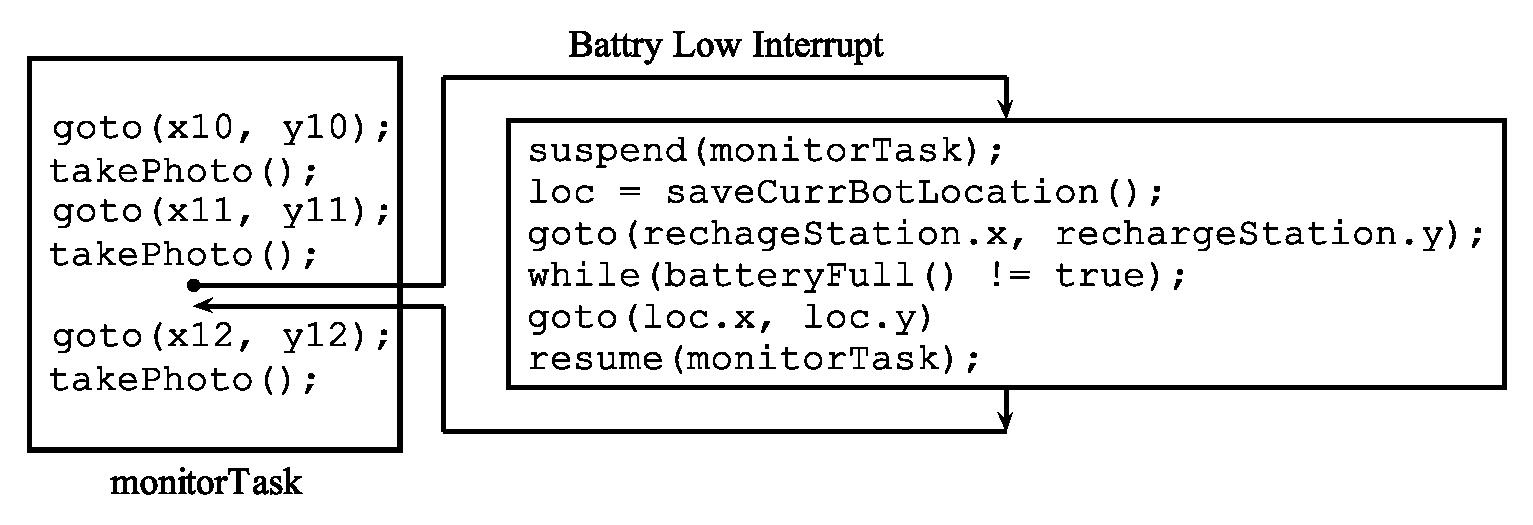
\includegraphics[scale=0.4]{./monitor}
}

\frame{\frametitle{Risk Mitigation}
 \structure{Risk \#4} Unauthorized user controls greenhouse
 
 \vspace{\baselineskip}
 Use secure network protocol and authenticate user before connection.
 }

\frame{\frametitle{Obeservations}
Problem of designing accurate and automated Bot guidance system is fundamental in nature for greenhouse applications.

\vspace{\baselineskip}
All future greenhouse projects can use this system to avoid costly or complex solutions.

\vspace{\baselineskip}
Applications who need very accurate Bot positioning just need to place \alert{extra checkpoints} at desired places.

\vspace{\baselineskip}
\hspace{0.4\textwidth} Thank You!
}

\frame{\frametitle{References}
\bibliography{sample}
}
\end{document}

